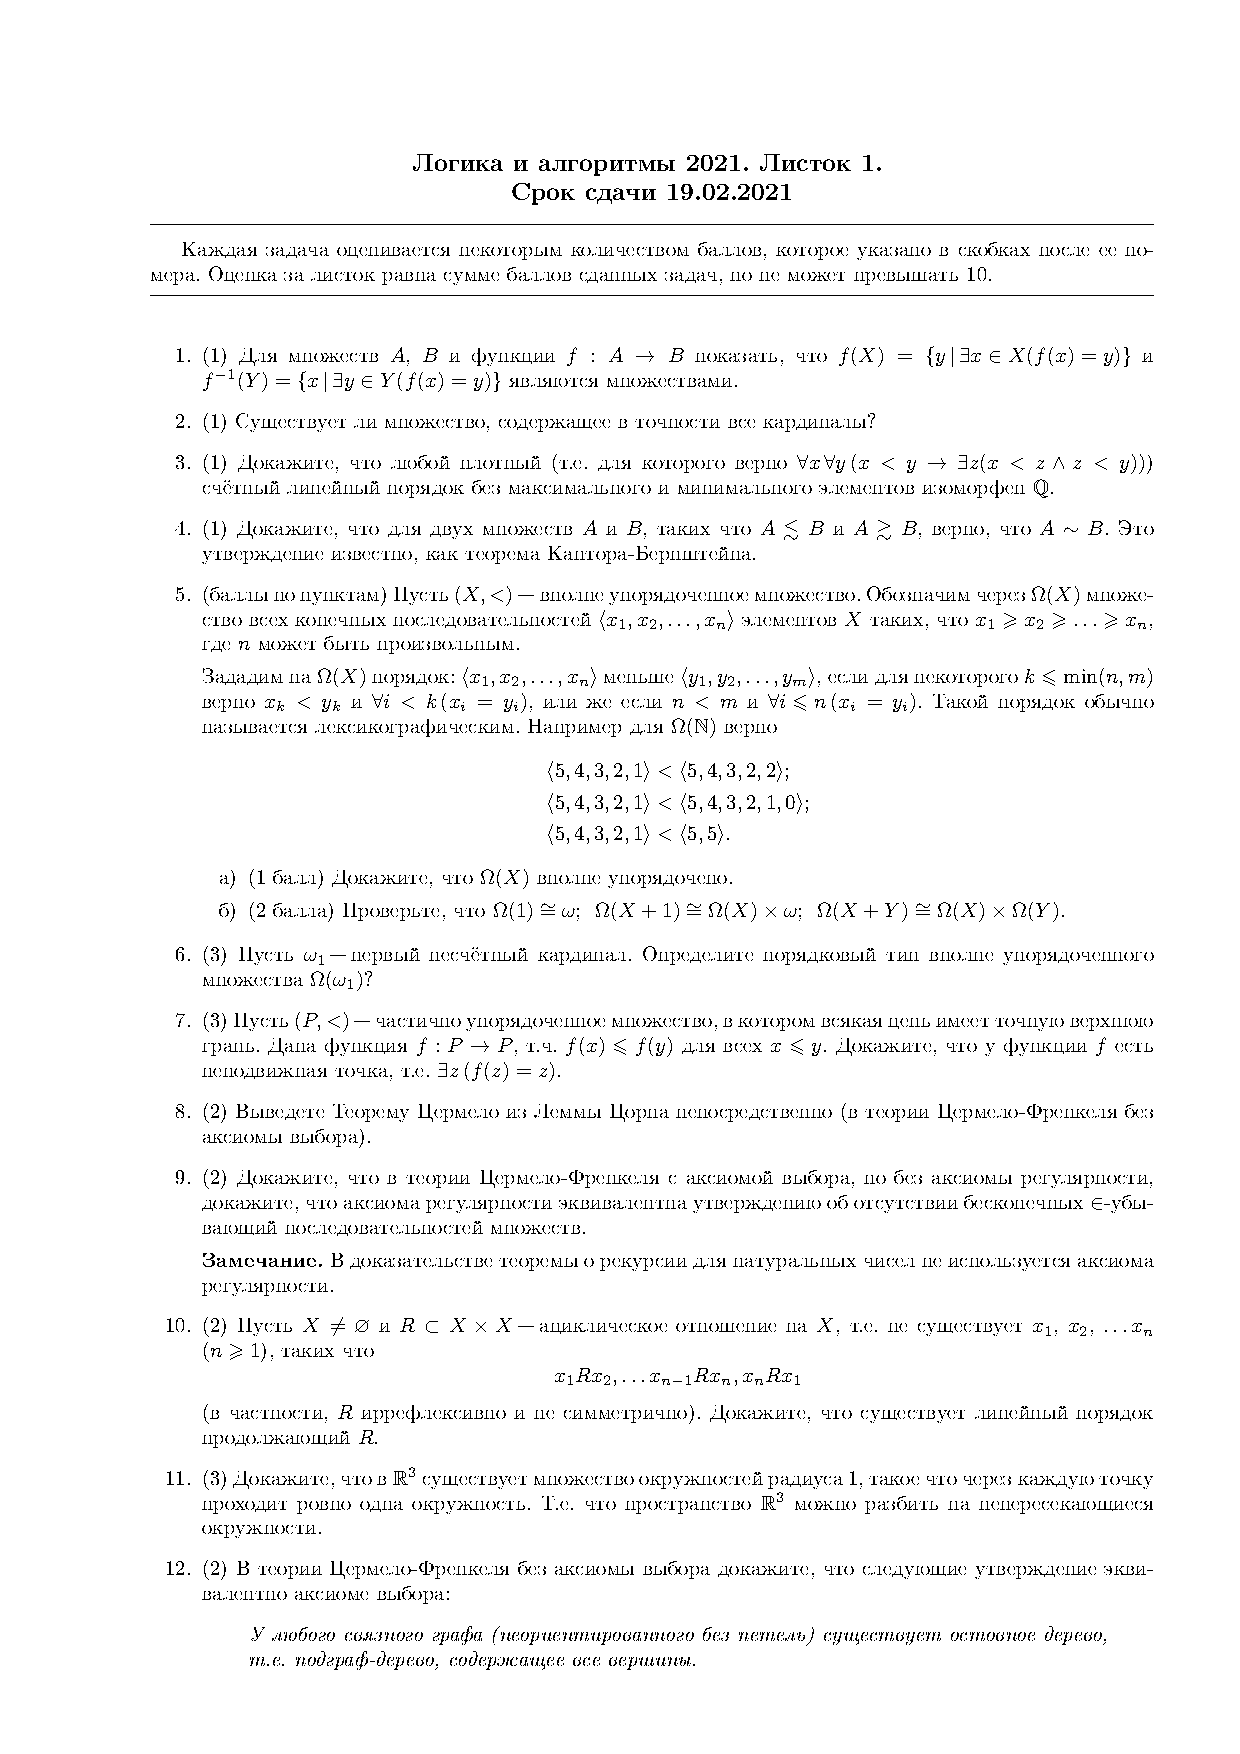
\includepdf[scale=1,pages=1]{Tasks/listok1}
\newpage
\section*{Решения}
\subsection*{Задача 1}
	\begin{figure}[!h]
		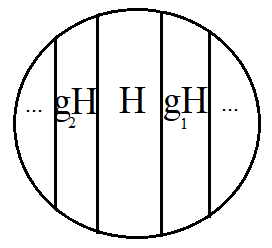
\includegraphics[width=0.65\linewidth]{Pic1}
	\end{figure}
	Вопспользуемся схемой аксиом подстановки. Пусть свойство $\varphi(x,y)$ - такое, что для любого множества $x$ айдется не более одного множества $y$, для которого $\varphi(x,y)$. Тогда для любого $X$ найдется множество $Y = \{y|\ \exists x \in X\ \varphi(x,y\}$\\
	Тогда $f^{-1}(y) = \{x|\ \exists y \in Y\ (f(x) = y)\}$ множество, теперь воспользуемся схемой аксиом выделения.\\
	Для любого свойства $\varphi$ и множества $Y$ существует множество $Z = \{x \in Y|\ \varphi(x)\}$. То есть для $X$ и свойства $\varphi(x) \leftrightarrow \exists y: f(x) = y$, существует множество $f^{-1}(Y) = \{x \in X|\ \varphi(x)\} = \{x \in X|\ \exists y: f(x) = y\}$
	\begin{comment}
	Схема аксиом выделения: для любого свойства множеств $\varphi$ и множества $\tilde{Y}$ существует множество $L = \{x \in Y\ |\ \varphi(x)\}$.\\
	Для $f(x) = \{y\ |\ \exists x \in X\ (f(x) = y)\}$ у нас:\\
	Свойство $\varphi(y):\ \exists x \in X:\ f(x) = y$,\\
	Множество $\tilde{Y} = B$
	\vskip 0.1in
	Тогда существует множество $L = \{y \in B\ |\ \varphi(y)\}$. Так как $f(x) \subset B$, это и есть $f(x)$.\\
	Для $f^{-1}(y) = \{x\ |\ \exists y \in Y\ (f(x) = y)\}$ есть:\\
	Свойство $\varphi(x):\ \exists y \in Y:\ f(x) = y,$\\
	Множество $\tilde{Y} = A$
	\vskip 0.1in
	Тогда существует множество $L = \{x \in A\ |\ \varphi(x)\}$, так как $f^{-1}(y) \subset A$, это и есть $f^{-1}(y)$
	\end{comment}
\vskip 0.4in

\subsection*{Задача 2}
	Допустим, существует множество всех кардиналов $A$, оно изоморфно кардиналу $\omega_N$. Существует $2^{\omega_N}$ множество всех подмножеств множества $\omega_N$, по теореме с семинара известно, что для любого множества $B: |B| \not\simeq |2^B|$. Тогда существует кардинал $\omega_{N_1}: \omega_{N_1} \simeq 2^{\omega_N}$, но $\omega_{N_1} \notin A$, так как $\omega_{N_1} < |A|$ -- противоречие.
	\begin{comment}
	Пусть $X$ -- множество всех кардиналов, $X = \{x_i,\ |\ x_i \text{ -- кардинал}\}$ и $\alpha = \bigcup X$. $\alpha$ -- ординал, покажем, что $\alpha$ -- кардинал, то есть не существует биекции $\alpha \to \beta,\ \forall \beta < \alpha$\\
	Докажем от противного. Пусть существует ординал $\beta$, такой что $f: \alpha \to \beta$ -- биекция. $\beta < \alpha = \bigcup X$, то есть $\exists n \in \gamma$ такой что $\beta \in x_n$\\
	Рассмотрим тогда ограничение $f|_{x_{n+1}}$. Это биекция на подмножество $\beta' \subset \beta \in x_n$. То есть $|x_{n+1}| \leqslant |x_n|$. Но кардинал не равномощен никакому меньшему ординалу. Противоречие, следовательно $\bigcup X$ -- кардинал.
	\end{comment}
\vskip 0.4in

\subsection*{Задача 3}
	$(A, <)$ счетно, плотно, линейно упорядочено, $\mathbb{Q}$ тоже. У обоих нет минимального или максимального элемента Докажем, что они изоморфны\\
	1) $\mathbb{Q}, A$ счетные, поэтому мы можем занумеровать их элементы\\
	2) Построим по шагам (элементов счетно, следовательно шагов тоже).\\
	Пусть мы построили множества $X,Y$ из $n$ элементов. Построение: возьмем элемент $\mathbb{Q}\backslash X$ или $Y \backslash A$ (пусть из $Y \backslash A$) и сравниваем его со всеми остальными элементами. Он или наименьший, или наибольший, или между $y_i, y_{i+1}$. Найдем элемент в $\mathbb{Q}\backslash X$, состоящий в таком же отношении с элементами $X$. Это можно сделать, так как $\mathbb{Q}$ плотно и не содержит минимального и максимального элемента. Теперь будем считать эти два элемента эквивалентными. На каждом шаге будем присоединять элемент из $\mathbb{Q}\backslash X$ или $Y \backslash A$ c элементом с наименьшим номером.
\vskip 0.4in

\subsection*{Задача 4}
	$(A, <)$ -- вполне упорядочено\\
	Пусть $B \subset A$, $(B, <_{B})$ -- полне упорядоченное множество. По теореме Кантора для любых двух вполне упорядоченных множеств одно изоморфно начальному отрезку другого.
	\begin{gather*}
		(B, <_{B}) \simeq [0,a)_{A}\\
		(A, <) \simeq [0,b)_{B}
	\end{gather*}
	Рассмотрим $f: A \to [0,b) \subset A$, это изоморфизм и $f$ сохраняет порядок.
	\vskip 0.1in
	Лемма из Лекции:\\
	Даны вполне упорядоченное множество $(A, <)$ и функция $f: A \to A$, сохраняющая порядок, тогда $a \leqslant f(a)\ \forall a \in A$\\
	В нашем случае это также выполнено, а следовательно $\forall a \in A: a \leqslant f(a)$\\
	$[0,b)_{B}$ по определению это подмножество $B \subset A$, такое что $\tilde{b} \in [0,b)_{B},\ \tilde{\tilde{b}} < \tilde{b} \Rightarrow \tilde{\tilde{b}} \in [0,b)_{B}$. У нас $\forall a \in A: a \leqslant f(a) \in [0,b)_{B}$, то есть $a \in [0,b)_{B}$. Значит, $A \subseteq [0,b)_{B} \subseteq A$, то есть $[0,b)_{B} = A$ и $B = A$, что и требовалось.
\vskip 0.4in

\subsection*{Задача 7}
	$(P, <)$ частично упорядочено, всякая цепь имеет точную верхнюю грань, следовательно по лемме Цорна $(P,<)$ имеет максимальный элемент.\\
	Зафиксируем $a \in P$ и построим функцию
	\begin{gather*}
		g: \gamma \to P\quad \gamma\text{ -- ординал, такой что не существует инъекции } \gamma \to P\\
		g =
		\begin{cases}
			g(0) = a\\
			g(\alpha + 1) = f(g(\alpha))\\
			g(\alpha) = \sup \{g(\beta): \beta < \alpha\}\quad \text{если } \alpha \text{ предельный ординал}
		\end{cases}
	\end{gather*}
	\begin{gather*}
		\forall x \leqslant y: f(x) \leqslant f(y) \Rightarrow \forall \alpha \leqslant \beta: g(\alpha) \leqslant g(\beta)\\
		\{g(\beta): \beta < \alpha\} \text{ -- цепь } \forall \alpha < \gamma
	\end{gather*}
	Пусть $g$ строго возрастает, следовательно оно инъективно, но $g: \gamma \to P$ не инъекция, откуда
	\begin{gather*}
		\exists \alpha < \beta < \gamma \text{, так что } g(\alpha) = g(\beta)\\
		g(\alpha) \leqslant g(\alpha + 1) \leqslant g(\beta) = g(\alpha)\qquad g(\alpha + 1) = f(g(\alpha))\\
		f(g(\alpha)) = g(\alpha)\\
		\exists z: f(z) = z
	\end{gather*}
	Покажем, что существует ординал $\alpha$, такой что не существует инъекции $\alpha \to P$\\
	$\alpha = \{\beta|\ \beta \text{ -- ординал такой, что существует инъекция } \beta \to P\}$ (то есть $\forall \beta \in \alpha\ \exists P'\subseteq P: \beta \simeq |P'|$)\\
	Возьмем инъекцию $g: \beta \to P$, некий $\gamma < \beta$ и $h: \gamma \to \beta$ -- включение. $g \circ h$ -- инъекция, следовательно $\gamma \in \alpha$, откуда $\beta \in \alpha, \gamma \in \beta$, то $\gamma \in \alpha$, тогда $\alpha$ -- транзитивно, его элементы тоже, а следовательно это ординал.\\
	Если существует инъекция $\alpha \to P$, то $\alpha \in \alpha$ -- противоречие.

\begin{comment}
	Докажем, что существует ординал $\alpha$ такой, что не существует инъекции $\alpha \to P$. $\alpha = \{ \beta\ |\ \beta \text{ -- ординал }, \exists \text{ инъекция } \beta \to P\}$. Покажем, что это множество. Пусть $W = \{(P', \leqslant): P'\subseteq P,\ \leqslant \text{вполне упорядоченное } P'\}$ -- вполне упорядоченные подмножества $P$. По теореме кантора $\forall w \in W$ соответствует единственный ординал $\beta w$, изоморфный $w$. $\{\beta|\ \exists w \in W: \beta = \beta w\}$ -- множество (последовательно объединяем $\beta w$ как множества). Это множество ординалов, которое изоморфно вполне упорядоченному подмножеству $P$. $\alpha$ -- множество ординалов, такое что существует инъекция $\beta \to P$ (или биекция $\beta \to f(\beta)$), инъекция индуцирует порядок, следовательно $\beta$ изоморфно подмножеству $P$, то есть это множество и есть $\alpha$.
	\vskip 0.1in
	Пусть $\beta \in \alpha$, тогда $\exists i: \beta \to P$ -- инъекция. Возьмем произвольный $\gamma < \beta$ и $l: \gamma \to \beta$ -- включение. Композиция инъекция -- инъекция, тогда $i \circ l: \gamma \to P$ -- инъекция. Значит $\gamma \in \alpha$. Получается $\beta \in \alpha,\ \gamma \in \beta$, откуда $\gamma \in \alpha$. Значит, $\alpha$ транзитивно. Все элементы $\alpha$ -- ординалы, то есть транзитивны, а следовательно $\alpha$ -- ординал. Если существует инъекция $\alpha \to P$, то $\alpha \in \alpha$ Но множество не может быть своим элементом, а следовательно не существует инъекции $\alpha \to P$.
	\vskip 0.2in
	$(P, <)$ -- частично упорядоченное множество, любая цепь которого имеет $\sup$, а следовательно по лемме Цорна $(P, <)$ содержит максимальный элемент.
	\begin{gather*}
		f: P \to P,\ f(x) \leqslant f(y)\ \forall x \leqslant y
	\end{gather*}
	Зафиксируем $p \in P$ и зададим $g: \gamma \to P$:
	\begin{gather*}
		g(0) = P\\
		g(\alpha + 1) = f(g(\alpha))\\
		g(\alpha) = \sup\{g(\beta):\ \beta < \alpha\}, \text{ если } \alpha \text{ -- пред. ординал}
	\end{gather*}
	$f(x) \leqslant f(y)\ \forall x \leqslant y$ по условию. Значит, $g(\alpha) \leqslant g(\beta)\ \forall \alpha \leqslant \beta$. Если $\alpha < \beta$, то $g(\alpha) \leqslant g(\text{любой ординал меньший } \alpha) \leqslant g(\beta)$.\\
	$\{g(\beta: \beta < \alpha\}$ -- цепь (линейно упорядоченное подмножество $P$) $\forall \alpha < \gamma$\\
	Предположим, что $g$ строго возрастает, тогда $g$ -- инъекция. То есть $\exists g: \alpha \to P$ нет.\\
	Тогда $\exists \alpha < \beta < \gamma$, такое что $g(\alpha) = g(\beta)$. Так как $\alpha + 1 \leqslant \beta$, $g(\alpha) \leqslant g(\alpha + 1) \leqslant g(\beta) = g(\alpha)$ и $g(\alpha + 1) = f(g(\alpha))$, то есть $f(g(\alpha)) = g(\alpha)$. Значит, $\exists z - g(\alpha)$, такое что $f(z) = z$.
\end{comment}
\vskip 0.4in

\subsection*{Задача 8}
	Вполне упорядоченное множество $(S, <_{S})$ назовем вполне упорядоченным подмножеством $X$, если $S \subset X$. Для данного множества $X$ рассмотрим совокупность $W(X)$ всех его вполне упорядоченных подмножеств. На $W(X)$ определим отношение строгого частичного порядка $\prec$ следующим образом:\\
	$(S, <_{S}) \prec (T, <_{T})$, если и только если $S \subset T$ -- собственный начальный отрезок $(T, <_{T})$, $<_S = <_T|_S$.
	\vskip 0.1in
	Порядок:\\
	транзитивность $(S,<_S) < (T, <_T),\ (T, <_T) < (M, <_M)$, следовательно $S \subset T$ -- собственный начальный отрезок $(T, <_T),\ <_S = <_T|_S,\ T \subset M$ -- собственный начальный отрезок $(M, <_M),\ <_T = <_M|_T$. Тогда $S \subset T \subset M,\ S$ -- собственный начальный отрезок $M$, $<_S = <_T|_S = <_{(M|T)|S}$, откуда $<_S = <_{M|T}$\\

	\vskip 0.1in

	Докажем, что $(W(X), \prec)$ удовлетворяет условию леммы Цорна. Рассмотрим любую цепь $C \subset W(X)$. Цепь -- подмножество $W(X)$, любые 2 элемента которого сравнимы, то есть среди любых двух элементов один является начальным отрезком другого, причем элементы -- это вполне упорядоченные подмножества $X$. Таким образом, цепи $C$ соответствуют возрастающая по включению цепь подмножеств $X$ и возрастающая по включению цепь бинарных отношений на этих множествах. Пусть $n$ -- объединение этой цепи подмножеств и $<_n$ -- цепи отношений.\\
	$<_n$ -- отношение линейного порядка на $n$ (все сравнимо). Каждое $(S_1, <_s) \in C$ -- начальный отрезок $(n, <_n)$. Тогда $(n, <_n)$ -- вполне упорядоченное подмножество $X$, следовательно это элемент $W(X)$,  также верхняя грань цепи $C$.\\
	Применим к $W(X)$ лемму Цорна. В $(W(X), <)$ найдется некоторый максимальный элемент $(M, <_M)$. Покажем, что $M = X$. Допустим это не так, тогда возьмем $a \in X \backslash M$ и продолжим порядок $<_M$ на $N = M \cup \{a\}$, считая $x <_N a,\ \forall x \in M$. Тогда $(N, <_N)$ -- вполне упорядоченное подмножество $X$, и $(M, <_M) \prec (N, <_N)$, но $(M, <_M)$ максимальный, следовательно $X$ -- это $(M, <_M)$, причем $(M, <_M)$ -- вполне упорядоченное множество. 

	%Докажем, что $(W(X), \prec)$ удовлетворяет условию леммы Цорна. Рассмотрим любую цепь $C \subset W(X)$. Цепи $C$ соответствует возратающая по включению цепь подмножеств $X$, а через $<_{U}$ -- объединение соответствующей цепи отношений. $<_{U}$ -- отношение линейного порядка на $U$ и $(S, <_{S}) \in C$ -- начальный отрезок $(U, <_{U})$. Отсюда получаем, что $(U, <_{U})$ -- вполне упорядоченное подмножество $X$. Таким образом, $(U, <_{U})$ -- элемент $W(X)$ и верхняя грань цепи $C$.\\
	%Применяя лемму Цорна получаем, что в $(W(X), \prec)$ найдется некоторый максимальный элемент $(M, <_{M})$. Тогда $M$ обязано совпадать со всем $X$: в противном случае мы можем взять $a \in X \backslash M$ и продолжить порядок $<_{M}$ на большее множество $N = M \cup \{a\}$ полягая $x <_{N} a$ для всех $x \in M$. Тогда $(N, <_{N})$ будет вполне упорядоченным подмножеством $X$ и $(M, <_{M}) \prec (N, <_{N})$, что противоречит максимальности $(M, <_{M})$.
\vskip 0.4in

\subsection*{Задача 9}
	(утверждение 1) Пусть $A$ -- множество, $A \ne \varnothing$, $R$ -- тотальное бинарное отношение на $A$. Тогда существует последовательность $(a_n)_{n \in \mathbb{N}}$, такая что $a_n R a_{n+1}\ \forall n \in \mathbb{N}$\\
	$R(a) \ne \varnothing\ \forall a \in A$ (отношение тотальное). $A$ разбивается на непересекающиеся классы эквивалентности, то есть $A$ -- семейство непустых классов эквивалентности. По аксиоме выбора существует функция $f:\ A \to A$, такая что $\forall a \in A:\ f(a) \in A$, откуда $f(a) \in R(a)$, так как $A$ разбито на классы эквивалентности. Значит, $\forall a \in A:\ a R f(a)$, так как $f(a) \in R(a)$
	\vskip 0.1in
	Зафиксируем $a \in A$ и рекурсивно зададим последовательность, то есть функцию из $M$:
	\begin{gather*}
	\begin{cases}
		a_0 = a\\
		a_{n+1} = f(a_n)
	\end{cases}
	\end{gather*}
	То есть последовательность выглядит так: $a,\ f(a),\ f(f(a)), \ldots$\\
	Аксиома регулярности равносильна отсутствию бесконечной $\in$-убывающей последовательности множеств.
	\vskip 0.1in
	($\Rightarrow$) Пусть существует такая последовательность, то есть $f$, определенная на $\mathbb{N}$. $f(n+1)$ -- это элемент $f(n)$ ля любого $n$ (так как последовательность $\in$-убывающая). Пусть $S = \{f(n)\ |\ n \in \mathbb{N}\}$ -- множество значений $f$. По аксиоме регулярности $\exists B \in S$, такое что $B \cap S = \varnothing$. По определению $S$, $B$ -- это $f(k)$ для какого-то $k \in \mathbb{N}$. $f(k)$ содержит $f(k+1)$, $f(k+1) \in S$. Тогда $f(k+1) \in f(k) \cap S$. Но в пересечении пустое множество -- противоречие, а следовательно такого $f$ не существует
	\vskip 0.1in
	($\Leftarrow$) Пусть $S \ne \varnothing$ является контрпримером к аксиоме регулярности, то есть $\forall s \in S:\ s \cap S \ne \varnothing$. Определим бинарное отношение $R$ на $S:\ aRb \Leftrightarrow b \in S \cap a \ne \varnothing$. Отношение тотальное, так как иначе $\exists s_1:\ \not\exists s_2 \in S:\ s_2 \in S \cap s_1$ -- противоречит определению $S$. По утверждению 1 существует последовательность $(a_n) \in S$, где $a_n R a_{n+1}\ \forall n \in \mathbb{N}$. Это бесконечная убывающая цепочка -- противоречие, такого $S$ не существует.
\vskip 0.4in

\subsection*{Задача 11}
	Используя теорему Цермело введем отношение полного порядка в $\mathbb{R}^3$\\
	Луч $\{\beta: \beta \leqslant \alpha\} < \{\beta: \beta \leqslant \gamma\}$, если $\alpha < \gamma$ и не существует луча равномощного $\mathbb{R}^3 \simeq 2^\omega$
	\vskip 0.1in
	Во вполне упорядоченном множестве существует минимальный элемент $a_0$, проведем через него окружность.
	\vskip 0.1in
	Затем воспользуемся трансфинитной индукцией: пусть $\forall \beta < \alpha$ проведены непересекающиеся окружности, тогда:\\
	1) точка $\alpha$ принадлежит одной из проведенных окружностей, в этом случае мы ничего не проводим\\
	2) точка $\alpha$ не принадлежит ни одной из проведенных окружностей, в этом случае построим окружность: Через $\alpha$ проходит континуум окружностей, а уже проведено $\leqslant \beta$ окружностей $\ne 2^{\omega}$. Выберем плоскость $A$, которая не содержит проведенных окружностей (это можно сделать, так как плоскостей континуум, а построенные окружности входят не более чем в $\beta$ плоскостей). Каждая окружность пересекает $A$ не более чем в 2 точках, а следовательно их меньше $2^\omega$. Проведем на $A$ семейство окружностей, касающихся в $\alpha$. Существует окружность, которую не пересекает ни одна построенная окружность (так как каждая из построенных окружностей пересекается не более чем с 2 из данного семейства).
	%потому что мы взяли минимальное отношение порядка, при котором R3 ~ континуум 2^w = объединение всех ординалов, меньших 2^w ~ объединение всех точек
	\begin{comment}
	Пусть $\phi$ -- ординал и $\mathbb{R}^3 = \{p_{\alpha}: \alpha < \phi\}$ будет некоторой нумерацией точек пространства. Определим единичную окружность $C_{\alpha}$, содержащей $p_{\alpha}$, через трансфинитную индукцию на $\alpha$, для некоторых $\alpha$ мы не будем ничего определять. Шаг индукции: пусть мы находимся на шаге $\alpha$ и какие-то окружности $\{C_{\beta}: \beta < \alpha\}$ уже определены. Если некоторые из них покрывают $p_{\alpha}$, мы ничего не добавляем. В противном случае выберем единичную окружность содержащую $p_{\alpha}$, которая не пересекается ни с одной из уже проведенных окружностей, для этого мы сперва выберем плоскость, прорходящую через $p_{\alpha}$ и не совпадающую с плоскостями уже имеющихся окружностей, это возможно, так как через $p_{\alpha}$ проходит континуум плоскостей, и менее чем континуум уже проведен. Пусть мы выбрали некую плоскость $K$, прошлые окружности пересекают $K$ менее чем в континуальном числе точек, и необходимо найти окружность в $K$, которая не проходит через точки уже проведенных окружностей. В $K$ континуум окружностей проходит через $p_{\alpha}$, и каждая из точек уже выбранных окружностей убирает ровно 2 окружности в плоскости $K$, а следовательно в $K$ можно провести окружность, не пересекающуюся ни с одной из уже проведенных.
	\end{comment}

\subsection*{Задача 12}
	(Выбор $\Rightarrow$ Дерево)\\
	Дан связанный граф, заметим что любой максимальный подграф без циклов будет остовным деревом, а существование такого подграфа следует из леммы Цорна (порядок введен по отоншению подграфа)
	\vskip 0.1in
	(Выбор $\Leftarrow$ Дерево)\\
	Дано непустое семейсто $(X_i)_{i \in I}$ непересекающихся непустых множеств, определим семейство одноэлементных множеств $(Y_i)_{i \in I}$ так, что $Y_i \notin X_j$ и какое-то $a \notin \bigcup_{i \in I}(X_i \cup \{Y_i\})$. Пусть $V := \{a\} \cup (\cup_{i \in I} (X_i \cup \{Y_i\}))$. Определим связный граф $G$ с вершинами $V$ таким образом: для каждого $i \in I$ и $x \in X_i$ свяжем(соединим ребром) $x$ с $Y_i$ и $a$. Определим остовное дерево $T$ графе $G$. Для каждого $i \in I$, каждый путь в $G$, проходящий через $Y_i$ и $a$, проходит через элемент $X_i$ (и для каждого $i$ элемент свой). Так как остовное дерево является связанным подграфом $G$, $T$ имеет хотя бы один путь, а так как в нем нет циклов, то такой путь ровно один. Пусть этот путь проходит через $x_i$ в $X_i$, тогда $(x_i)_{i \in I}$ Принадлежит $\prod_{i \in I}X_i$.

\begin{comment}
	Бесконечный граф является связным, если для каждой пары вершин есть конечный путь с концами в этих вершинах.\\
	Деревья внутри графа могут быть частично упорядочены отношением подграфа. Любая бесконечная цепь имеет верхнюю грань (объединение деревьев в цепочке). Тогда выполнены условия леммы Цорна, значит частичный порядок имеет максимальный элемент, это и есть остовное дерево.
	\vskip 0.1in
	Пусть остовное дерево существует.\\
	Аксиома выбора: для любого семейства $\{X_i\}_{i \in I}$ непустых множеств существует $f: I \to \bigcup X$, (остовное дерево $\mapsto$ функция выбора)\\
	Построим связный граф $G$ с набором вершин $U$. $V = \{r\} \cup (\bigcup_{i \in I} (X_i \cup \{O_i\}))$, где $\{X_i\}_{i \in I}$ -- семейство непересекающихся непустых множеств, $\{O_i\}_{i \in I}$ семейство, такое что $O_i \notin X_j$, $r \in \bigcup_{i \in I}(X_i \cup \{O_i\})$\\
	$\forall i \in I\ x \in X_i$ соединим $x$ и $O_i$ или $r$. Рассмотрим остовное дерево в графе $G$. $\forall i \in I$ и для любого пути в $G$ соединим $O_i$ и $r$. $(X_i)_{i \in I}$ -- попарно неперсекающиеся непустые множества. $O_i := (X,i)_{\forall }$
\end{comment}